\section{Diseño}
\subsection{Diseño de la arquitectura del sistema}

\begin{figure}[!h]
    \centering
    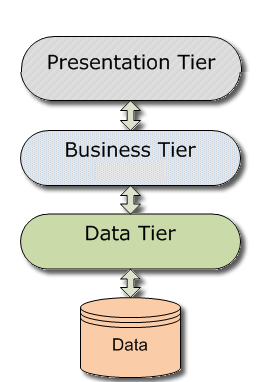
\includegraphics[]{images/multilevel-architecture.png}
    \caption{Arquitectura multinivel}
    \label{multilevel-architecture}
\end{figure}

Se ha usado una arquitectura multinivel partiendo de la base de datos que nos provee
\textit{firebase} a la cual se conecta la aplicación a través de su API. Esta API
se consume desde la aplicación con los proveedores de los que dispone Ionic, para
posteriormente mostrar la información resultante en la capa de presentación.
El problema ha sido a la hora de añadir nueva lógica referente a la aplicación.
Esta API no permite ser modificada y se ha tenido que incluir cierta lógica de
negocio en la propia aplicación. Es por ello que para el futuro si se quiere
implementar este prototipo y que sea escalable, se tendría que desarrollar una
API propia donde alojar toda la lógica de negocio.

\medskip
Con ello se aprovecharía de mejor forma las ventajas de esta arquitectura. Como
puede ser la fácil escalabilidad debido a que pueden haber varios clientes
consumiendo de la misma lógica. Y en caso de que la lógica cambie, no tenga un
mantenimiento complejo debido a que se encuentra toda en un lugar centralizado.
Por otro lado disponer de esta API supondría un ahorro de recursos en el cliente,
porque este no tendría que hacer cálculos referentes a la lógica del negocio.

\subsection{Diseño de la base de datos}
\medskip
Para el registro de usuarios se ha usado el módulo de autenticación
del que dispone esta misma plataforma, el cual permite el registro
de usuarios por múltiples vías si así lo quisiéramos, guardan de
forma segura las contraseñas e incorpora un sistema de verificación
de correo en el momento del registro. Es por ello que se ha tenido
que crear un objeto en la base de datos, a parte del existente,
para incluir datos personales que usando este módulo no nos permitían
guardar. Para ello se ha creado un grupo llamado \textit{users} donde
crear objetos de nombre, el identificador único, generados en el
momento del registro de cada usuario y dentro de este el resto de
datos que nos han sido necesarios.

\medskip
\begin{figure}
    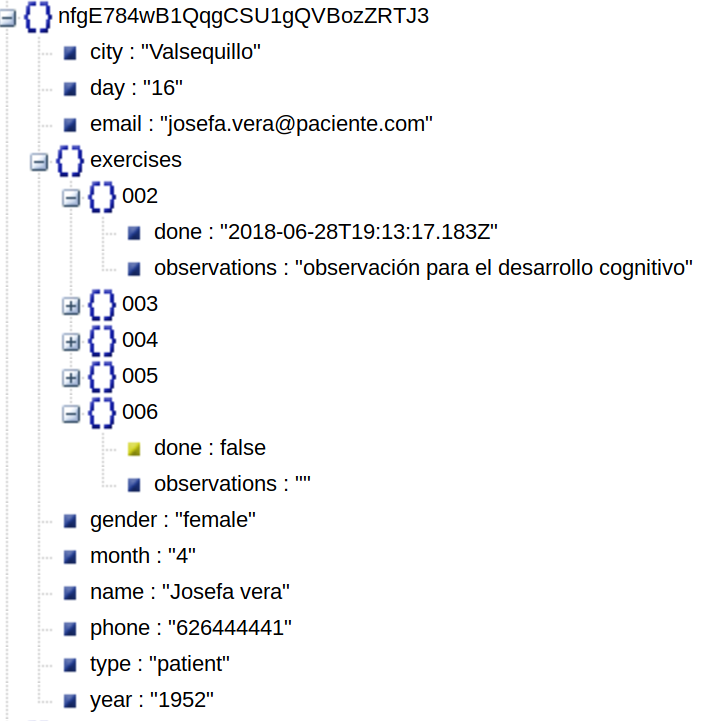
\includegraphics[width=\linewidth]{./images/database/user-patient.png}
    \caption{Estructura en la base de datos del objeto: usuarios (paciente)}
    \label{user-patient}
\end{figure}

Como se puede ver en la \textbf{figura \ref{user-patient}},
los usuarios comparten parámetros comunes de los cuales solamente los que
se explicarán a continuación pueden generar duda de su utilidad o uso que se
le ha podido dar. Es el caso de \textit{city}, hace referencia a la ciudad de
nacimiento del usuario y por otro lado el trío \textit{day-month-year} los
cuales forman la fecha de nacimiento del usuario en cuestión.
En este caso el usuario tiene asignados cinco ejercicios dentro del objeto
\textit{exercise} a los cuales se les "referencia" guardando como clave su ID.
Dentro de este objeto cada ejercicio tiene un campo observaciones
(\textit{observatios}) y un campo completado (\textit{done}) donde se guarda
la fecha y hora en la que se completó un ejercicio.

\medskip
\begin{figure}
    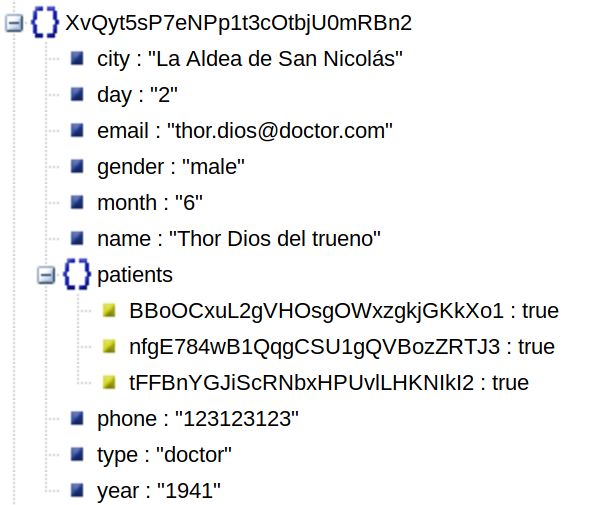
\includegraphics[width=\linewidth]{./images/database/users-doctor-database.png}
    \caption{Estructura en la base de datos del objeto: usuarios (doctor)}
    \label{usuario-doctor}
\end{figure}

En caso de ser un usuario de tipo doctor este tendrá un objeto en el que
guarda los identificadores de sus pacientes asignados. Como se puede ver
en la \textbf{figura \ref{usuario-doctor}} estos pacientes tienen asignados
una fecha y hora, correspondiente a la última hora en la que se visitó su
perfil.

\medskip
\begin{figure}
    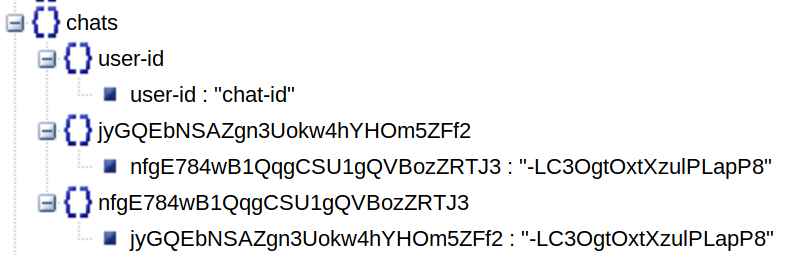
\includegraphics[width=\linewidth]{./images/database/chats-database.png}
    \caption{Estructura en la base de datos del objeto: chats}
    \label{chat}
\end{figure}

Para no hacer grandes cantidades de peticiones sin necesidad
se ha creado un objeto \textit{chats}, el cual se puede ver en la
\textbf{figura \ref{chat}}. Para explicar mejor como están estructurados
estos datos se pondrá un ejemplo. Si un usuario \textbf{A} tiene un chat
iniciado con un usuario \textbf{B} en la base de datos en la parte de chat
aparecerá la siguiente información:

\smallskip
\textit{chats/ ID-usuario-A/ [ID-usuario-B: ID-chat]}

\smallskip
\textit{chats/ ID-usuario-B/ [ID-usuario-A: ID-chat]}

\smallskip
En caso de que un tercer usuario \textbf{C} inicie un chat con \textbf{A}
aparecerá una nueva entrada y quedará de la siguiente forma la base de datos:

\smallskip
\textit{chats/ ID-usuario-A/ [ID-usuario-B: ID-chat], [ID-usuario-C: ID-chat]}

\smallskip
\textit{chats/ID-usuario-B/[ID-usuario-A: ID-chat]}

\smallskip
\textit{chats/ID-usuario-C/[ID-usuario-A: ID-chat]}

\smallskip
Como se ha dicho esto se ha realizado de esta forma para ahorrar
tener que traer todos los
mensajes del chat en caso de que un usuario solo quiera visualizar con
que personas tiene un chat abierto, de esta forma solo hará una petición
al objeto con su identificador y este le devolverá los ID de los usuarios
con los que mantiene la conversación y el ID del chat en cuestión si quiere
obtener los mensajes.

\medskip
\begin{figure}
    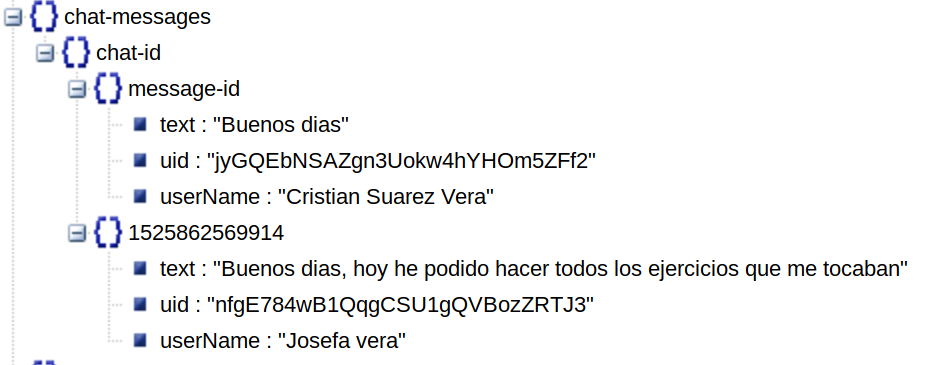
\includegraphics[width=\linewidth]{./images/database/chat-messages-database.png}
    \caption{Estructura en la base de datos del objeto: mensajes del chat}
    \label{mensajes-del-chat}
\end{figure}

A raíz de la implementación anterior se ha tenido que crear el objeto
que muestra la \textbf{figura \ref{mensajes-del-chat}}, este tiene como
objetivo almacenar todos los mensajes de los chats entre los distintos
usuarios. Cada chat tiene su identificador único con el que se crea el
objeto y dentro de este un identificador de mensaje el cual internamente
tiene el mensaje que ha sido enviado, el identificador del usuario que
ha enviado el mensaje y el nombre completo del usuario que ha enviado
el mensaje. Este último parámetro puede parecer redundante pero nos
ahorra posteriormente, a la hora de mostrar los mensajes, tener que hacer
una petición al servidor para obtener este dato.

\medskip
\begin{figure}
    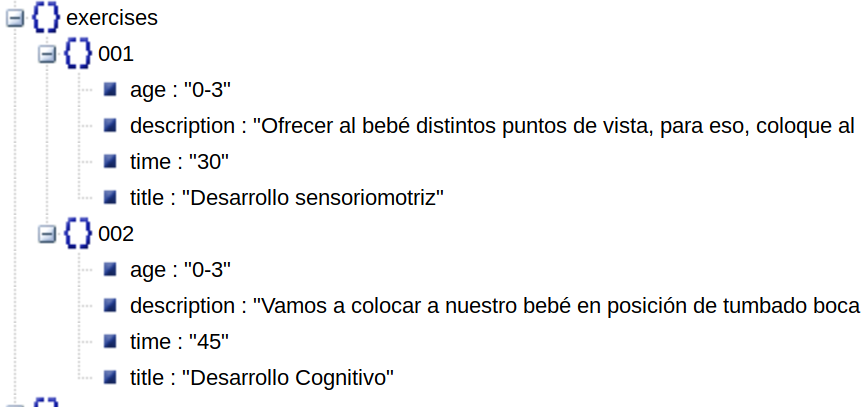
\includegraphics[width=\linewidth]{./images/database/exercises-database.png}
    \caption{Estructura en la base de datos del objeto: ejercicios}
    \label{ejercicios}
\end{figure}

Por último en la \textbf{figura \ref{ejercicios}} se ve
como se ha creado el objeto para los ejercicios. En él se almacena la información
referente a cada ejercicio como puede ser la edad recomendada del ejercicio,
la descripción del mismo, el tiempo medio que se tarda en realizarlo y el
título que este tiene. Además todo ello está bajo un objeto que tiene como
nombre un identificador único para el ejercicio.

\subsection{Almacenamiento de contenido multimedia}

Para almacenar todo el contenido multimedia referente a los ejercicios se ha
decidido usar \textit{firebsae storage}. Un servicio que nos permite guardar
todas las ilustraciones y vídeos referentes al prototipo y acceder a ellos en
todo momento. Este almacenamiento se ha organizado de tal forma que disponemos
de un directorio principal y dentro de este existen directorios con el nombre
del ejercicio al que corresponde el contenido. Cada uno de ellos tiene en su
interior todo el contenido multimedia referente al ejercicio.

\subsection{Diseño arquitectónico}

En este apartado se ha usado el diseño propio del que dispone Ionic. Este consta
de vista y proveedor. Los proveedores acceden a la información disponible en el
servido, le dan formato y la envían a la vista. En este caso en estos proveedores
contienen algo de lógica del negocio. Esto ocurre porque no se ha podido modificar
la API que ofrece firebase. La vista recibirá la información preparada por los
proveedores y la mostrará al usuario para que haga uso de ella.